%%
%% Class homework & solution template for latex
%% Alex Ihler
%%
\documentclass[twoside,11pt]{article}
\usepackage{amsmath,amsfonts,amssymb,amsthm}
\usepackage{graphicx,color}
\usepackage{verbatim,url}
\usepackage{listings}
\usepackage{upquote}
\usepackage[T1]{fontenc}
%\usepackage{lmodern}
\usepackage[scaled]{beramono}
%\usepackage{textcomp}

% Directories for other source files and images
\newcommand{\bibtexdir}{../bib}
\newcommand{\figdir}{fig}

\newcommand{\E}{\mathrm{E}}
\newcommand{\Var}{\mathrm{Var}}
\newcommand{\N}{\mathcal{N}}
\newcommand{\matlab}{{\sc Matlab}\ }

\setlength{\textheight}{9in} \setlength{\textwidth}{6.5in}
\setlength{\oddsidemargin}{-.25in}  % Centers text.
\setlength{\evensidemargin}{-.25in} %
\setlength{\topmargin}{0in} %
\setlength{\headheight}{0in} %
\setlength{\headsep}{0in} %

\renewcommand{\labelenumi}{(\alph{enumi})}
\renewcommand{\labelenumii}{(\arabic{enumii})}

\theoremstyle{definition}
\newtheorem{MatEx}{M{\scriptsize{ATLAB}} Usage Example}

\definecolor{comments}{rgb}{0,.5,0}
\definecolor{backgnd}{rgb}{.95,.95,.95}
\definecolor{string}{rgb}{.2,.2,.2}
\lstset{language=Matlab}
\lstset{basicstyle=\small\ttfamily,
        mathescape=true,
        emptylines=1, showlines=true,
        backgroundcolor=\color{backgnd},
        commentstyle=\color{comments}\ttfamily, %\rmfamily,
        stringstyle=\color{string}\ttfamily,
        keywordstyle=\ttfamily, %\normalfont,
        showstringspaces=false}
\newcommand{\matp}{\mathbf{\gg}}




\begin{document}

\centerline{\Large Homework 3}
\centerline{Zachary DeStefano, 15247592}
\centerline{CS 273A: Winter 2015}
\centerline{\bf Due: January 27, 2015}

\section*{Problem 1}

\subsection*{Part a}

This is the plot of class 0 versus class 1, which is linearly separable. \\
\begin{figure}[h]
\centering
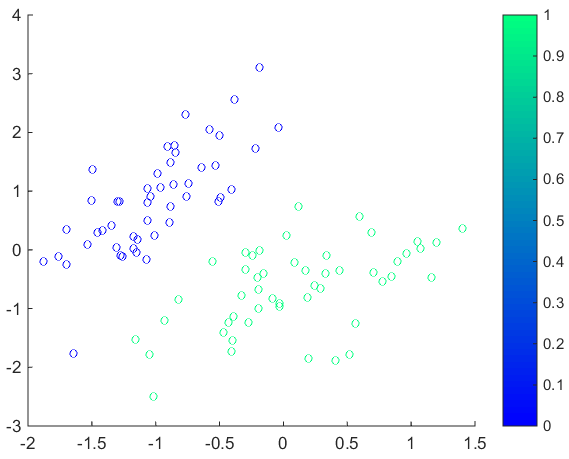
\includegraphics[width=4 in]{prob1aPlot1.png}
\caption{Class 0 and Class 1 Points}
\end{figure}
\newpage
This is the plot of class 1 versus class 2, which is not linearly separable. \\
\begin{figure}[h]
\centering
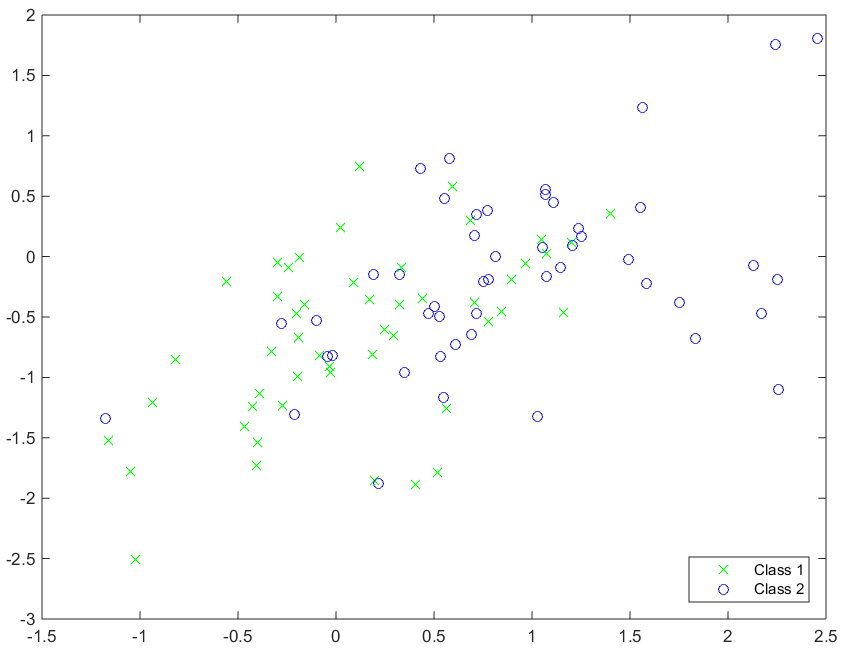
\includegraphics[width=4 in]{prob1aPlot2.png}
\caption{Class 1 and Class 2 Points}
\end{figure}
\\
Here is the code to complete part a
\lstinputlisting[firstline=1, lastline=22]{prob1.m}
\newpage
\subsection*{Part b}

Here is the plot of class 0 and class 1 along with the specified decision boundary\\
\\
\begin{figure}[h]
\centering
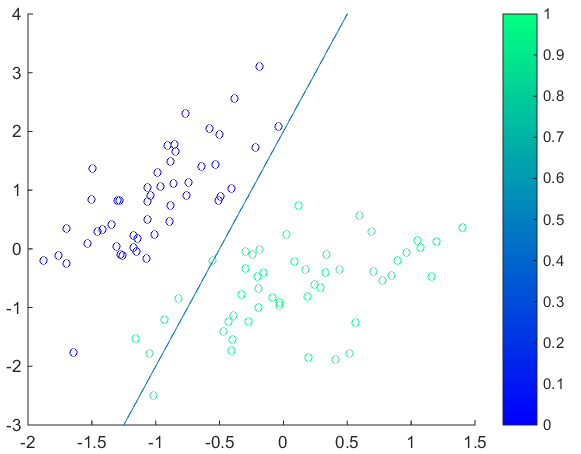
\includegraphics[width=4 in]{prob1bPlot1.png}
\caption{Class 0 and Class 1 points along with the sample decision boundary}
\end{figure}
\newpage
Here is the plot of class 1 and class 2 along with that decision boundary\\
\\
\begin{figure}[h]
\centering
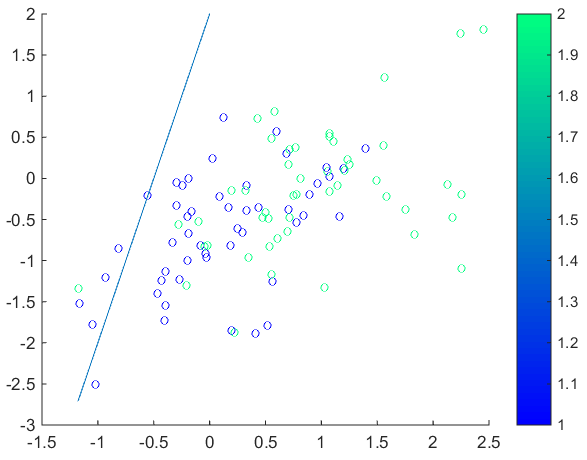
\includegraphics[width=4 in]{prob1bPlot2.png}
\caption{Class 1 and Class 2 points along with the sample decision boundary}
\end{figure}
\\
Here is the code for plot2DLinear
\lstinputlisting[firstline=1, lastline=21]{@logisticClassify2/plot2DLinear.m}
\newpage
Here is the code to complete part b. It does rely on some of the variables from the part a code.
\lstinputlisting[firstline=24, lastline=46]{prob1.m}

\subsection*{Part c}

I got an error rate of $0.0505$ for data set A\\
 and an error rate of $0.4646$ for data set B.\\
\\
Here is the code for predict.m
\lstinputlisting[firstline=1, lastline=20]{@logisticClassify2/predict.m}
\newpage
Here is the code to compute the error rates for part C. It relies on the code for Part B.
\lstinputlisting[firstline=46, lastline=57]{prob1.m}

\subsection*{Part d}

We will use the following identity:
\[
\sigma'(z) = \sigma(z)(1-\sigma(z))
\]
When we first take the derivative, we end up with
\[
\frac{\partial J_j}{\partial \theta_i} = -y^{(j)} (1-\sigma(z)) z' + (1-y^{(j)}) \sigma(z) z' + 2 \alpha \theta_i
\]
We know that $z' = \frac{\partial z}{\partial \theta_i}= x_i^{(j)}$ thus expanding terms we get
\[
\frac{\partial J_j}{\partial \theta_i} = -y^{(j)}x_i^{(j)} + x_i^{(j)}\sigma(z)y^{(j)} + \sigma(z) x_i^{(j)} -y^{(j)} \sigma(z) x_i^{(j)} + 2 \alpha \theta_i
\]
Cancelling out terms and then putting the $x_i^{(j)}$ factors together, we get
\[
\frac{\partial J_j}{\partial \theta_i} = x_i^{(j)} (\sigma(z) - y^{(j)} ) + 2 \alpha \theta_i
\]
The gradient vector $\nabla J_j(\theta)$ will be as follows
\[
[\frac{\partial J_j}{\partial \theta_1} \frac{\partial J_j}{\partial \theta_2} ... \frac{\partial J_j}{\partial \theta_d}]
\]
\newpage
\subsection*{Part e}

Here is the code for train.m
\lstinputlisting[firstline=1, lastline=117]{@logisticClassify2/train.m}

\newpage

\subsection*{Part f}

For Data Set A, the convergence seemed to work pretty well with the step size already given that starts at 1 and then decreases with each iteration, so I did not touch the step size. I decided to look at number of iterations and stop tolerance. After about 30-40 iterations, it seemed to be converging. When I zoomed in, however, I noticed that the error rate was still decreasing. I decided then to do 100 iterations total and set the stop tolerance really low at 0.0000001 in order to get the error rate as low as possible. In the end, all the points seemed to be classified perfectly which is what we wanted here since the data was linearly separable. \\
\\
Here is the surrogate loss and error rate plot for Data Set A\\
\begin{figure}[h]
\centering
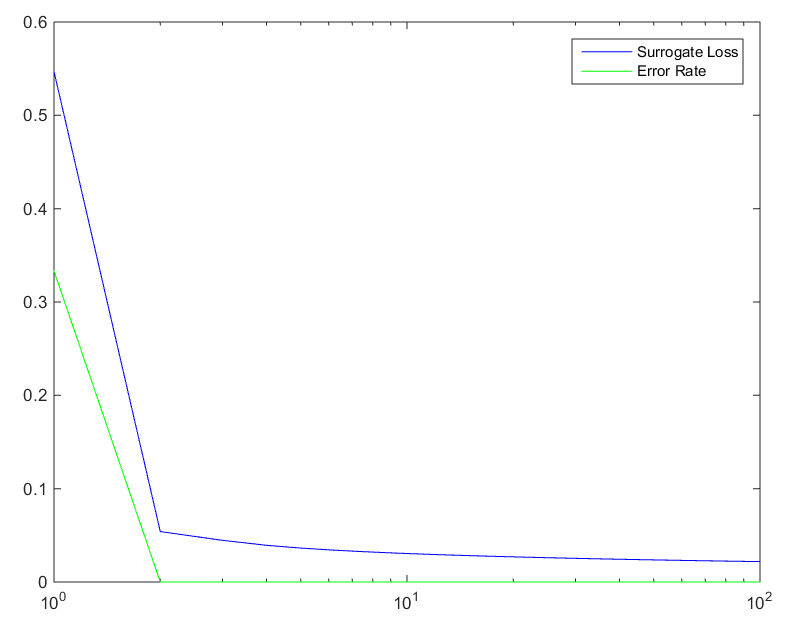
\includegraphics[width=5 in]{prob1fPlotA1.png}
\caption{The surrogate loss and error rate as function of number of iterations}
\end{figure}

\newpage
Here is the classification plot using the final weights computed to attempt to separate Data Set A.\\

\begin{figure}[h]
\centering
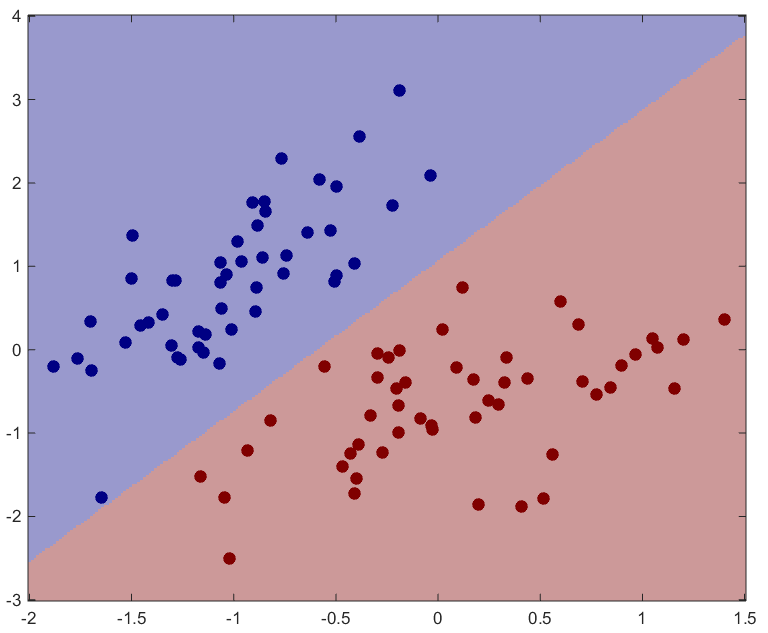
\includegraphics[width=5 in]{prob1fPlotA2.png}
\caption{The predicted and actual classification of points. In this case, they were all predicted correctly!}
\end{figure}

\newpage
For Data Set B, the convergence seemed to work well also so I left the step size as it was for data set A. It did take longer for the surrogate loss to converge, so I set the max number of iterations to 1000 and it was near converenge around 400 iterations. I decided to set the stop tolerance to the same value at 0.0000001 in order to get the error rate as low as possible. In this case, it did not execute all iterations before the stop tolerance was reached. There were around 800 iterations and then the stop tolerance criteria was met. The error rate however was still somewhat high. This is likely due to the fact that the data is not linearly separable so we reached a point where the error rate was as low as we could possibly make it. \\
\\
Here is the surrogate loss and error rate plot for Data Set B\\
\begin{figure}[h]
\centering
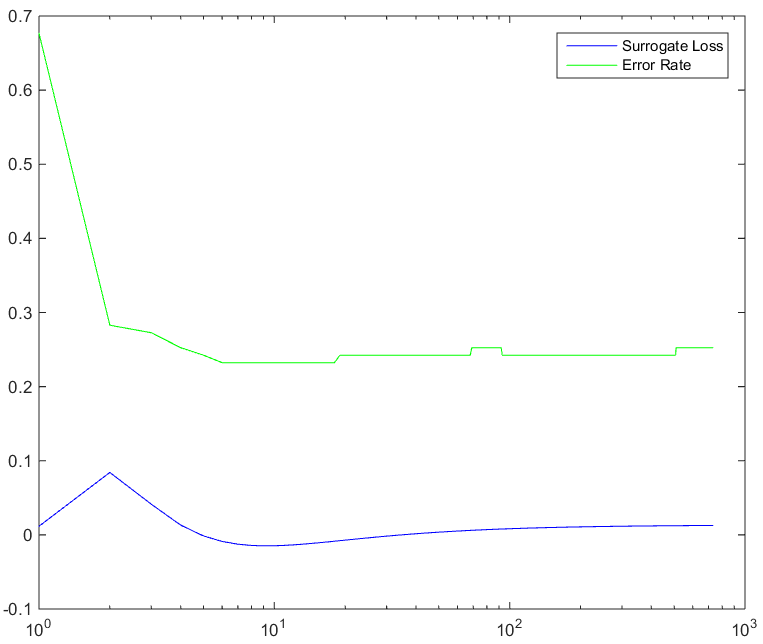
\includegraphics[width=5 in]{prob1fPlotB1.png}
\caption{The surrogate loss and error rate as function of number of iterations}
\end{figure}

\newpage

Here is the classification plot using the final weights computed to attempt to separate Data Set B\\

\begin{figure}[h]
\centering
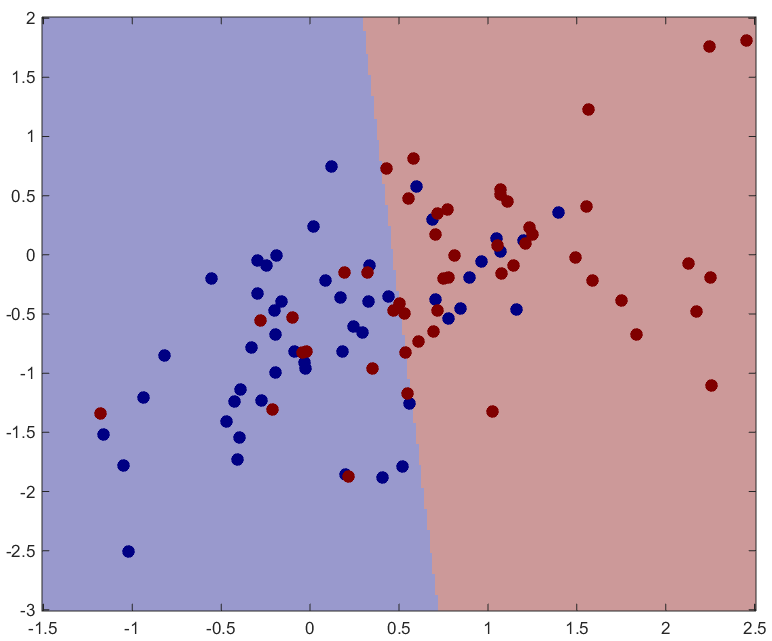
\includegraphics[width=5 in]{prob1fPlotB2.png}
\caption{The predicted and actual classification of points}
\end{figure}

As part as code is concered, in addition to the train.m function that I listed in part e as well as the code from part a to initialize the variables, I also used the following script to call the train functions and generate the classification plot.
\lstinputlisting[firstline=61, lastline=75]{prob1.m}

\newpage

\section*{Problem 2}

\subsection*{Part a}

This equation describes a vertical line through the points.\\
It will thus easily separate the points in (a) and (b).\\
\\
For the points in (c), if the points (2,2) and (6,4) had one class and the point (4,8) was of a different class, then a vertical line could not separate them.\\
\\
Thus the most points that this one could shatter is 2\\
The VC dimension is thus estimated at 2

\subsection*{Part b}

This equation describes a circle with an arbitrary center and radius\\
It will thus easily separate points in (a) and (b)\\
\\
With (c), if all points have the same class then of course this equation will separate them. \\
The other case to consider is one point has one class and the other two points have another class. \\
In this case, you can draw a small circle around the one point and now you have successfully separated the classes.\\
\\
With (d), this equation can technically separate them.\\
If zero points are in a class, then this is trivial. \\
If 1 point is in a class, so 3 in another class, then we can draw a circle around the point.\\
If there are 2 points in a class, then no matter which two you pick for a class, you can actually draw a circle around those two points or the other two points and you have a successful classification. \\
This only happened due to these particular points and how they were spaced. If I shifted one of the points closer to the other points, then there would be no way to separate them. \\
\\
Even though we could shatter 4 points, it only seems like we could reliably shatter 3 points in general.\\
The VC dimension is thus estimated at 3.

\subsection*{Part c}

This is a line that is centered at the origin and not horizontal since then $a \neq 0$. \\
\\
It can easily separate points in (a) and (b)\\
\\
With (c), if the points (6,4) and (4,8) had one class and the point (2,2) was part of another class, then there would be no way to separate them using a line at the origin. If it were possible to separate them, then we would be able to split the number line in two and put $\frac{2}{3}$ and 2 into one part while putting 1 into the other part.\\
\\
Thus, the most number of points this equation can shatter is 2\\
The VC dimension is thus 2

\end{document}
